\documentclass[lettersize,journal]{IEEEtran}
\usepackage{amsmath,amsfonts}
\usepackage{algorithmic}
\usepackage{array}
\usepackage[caption=false,font=normalsize,labelfont=sf,textfont=sf]{subfig}
\usepackage{textcomp}
\usepackage{stfloats}
\usepackage{url}
\usepackage{verbatim}
\usepackage{graphicx}
\hyphenation{op-tical net-works semi-conduc-tor IEEE-Xplore}
\def\BibTeX{{\rm B\kern-.05em{\sc i\kern-.025em b}\kern-.08em
    T\kern-.1667em\lower.7ex\hbox{E}\kern-.125emX}}
\usepackage{balance}


\usepackage{cite}
\usepackage{amsmath,amssymb,amsfonts}
\usepackage{algorithmic}
\usepackage{graphicx}
\usepackage{textcomp}
\usepackage{xcolor}
\def\BibTeX{{\rm B\kern-.05em{\sc i\kern-.025em b}\kern-.08em
    T\kern-.1667em\lower.7ex\hbox{E}\kern-.125emX}}


\usepackage{float}

\usepackage{textcomp}  % Copyright, trademark


\usepackage{subcaption}
%---------------------------------mohammed
% \usepackage{glossaries}
\usepackage[acronym]{glossaries}
\renewcommand*{\glstextformat}[1]{\textcolor{green}{#1}} 

\loadglsentries{contents/acronyms}%modify_path
\makeglossaries
\glsaddall

\usepackage{hyperref}
\hypersetup{
    colorlinks,
    linkcolor={red!50!red},
    citecolor={red!50!red},
    urlcolor={red!80!red}
}
\newcommand{\reffig}[1]{\autoref{#1}}
\newcommand{\reftab}[1]{\autoref{#1}}
\newcommand{\refeq}[1]{(\autoref{#1}), }%\eqref
% \newcommand{\refeq}[1]{(\eqref{#1}), }%\eqref
% \newcommand{\cite}[1]{\cite{#1}}
\newcommand{\citeN}[1]{}
% \usepackage{float}
% \usepackage{longtable}
% \usepackage{multicol}
% \setlength{\columnsep}{1cm}
\usepackage{soul}
\newcommand{\hlw}[1]{\hl{#1}}

% \usepackage{lipsum}  


\usepackage{multirow}

% \def\textsubscript#1{\ensuremath{_{\mbox{\textscale{.6}{#1}}}}}


% \usepackage{float}
\begin{document}


\title{ Integration of Server- and Embedded System-Based Technology for Dysphagia Data Collection
\author{\IEEEauthorblockN{Nikolay Nechaev, Andrey Somov}

% \IEEEauthorblockA{$^{1}$\textit{Skolkovo Institute of Science and Technology, Russia} \\
% %Moscow, Russia \\
% %julia.orlova@skoltech.ru
% }

% \IEEEauthorblockA{$^{2}$\textit{xxxxxxxxxxxxx}}


\thanks{

}
}
}
\markboth{}%
{}

\maketitle


\section{Introduction}

According to Bloem \textit{et al.} \cite{bloem2021PD}, Parkinson's disease is a
neurodegenerative disorder with varying symptoms, including
radykinesia, tremor, depression, constipation, distributed sleep, and cognitive decline
As of 2016, there were 6.1 million people affected by the condition,
with that number increasing in the past two decades.
One of the Parkinson's disease's symptoms, \textit{dysphagia}, is associated with the
death risk of patients experiencing it.


Dysphagia, or swallowing dysfunction, refers to the difficulty or discomfort experienced while swallowing\footnote{\url{https://www.hopkinsmedicine.org/health/conditions-and-diseases/swallowing-disorders}}. It can affect people of all ages and may be caused by various factors. The severity of dysphagia may vary, ranging from mild discomfort or difficulty to a complete inability to swallow\footnote{\url{https://www.nnuh.nhs.uk/departments/speech-and-language-therapy/swallowing/instrumental-swallow-assessment/}}. Dysphagia can lead to reduced food and fluid intake, longer meal times, and less enjoyment of eating and drinking. It may also cause people to avoid social activities such as dining out. Additionally, dysphagia can lead to food or drink entering the airway instead of the esophagus, passing the vocal cords, and entering the lungs, which can be potentially life-threatening. Other consequences include malnutrition, aspiration pneumonia, and even death.
\\


There are several methods to detect Dysphagia. The gold standards are \gls{VFSS} and \gls{FEES}\footnote{\url{https://www.hopkinsmedicine.org/health/treatment-tests-and-therapies/fiberoptic-evaluation-ofFEES}}. \gls{VFSS} is an evaluation of swallowing function performed using a video x-ray. During this assessment, a Speech and Language Therapist will provide a patient with food and drinks of varying consistency and observe as they swallow it. This enables a therapist to identify and analyze issues with the patient's swallowing, including food going in the wrong direction. \gls{FEES}\footnote{\url{https://swallowingdisorderfoundation.com/patient-videos/}} is another type of swallow assessment that involves inserting a camera through one's nose to view their throat. A therapist will offer food and drinks, and observe the swallowing process. Similar to \gls{VFSS}, the therapist can detect problems and see if anything is going towards the lungs.


\gls{VFSS} is an invasive procedure that involves radiation exposure~\cite{morishima2016estimation} and carries the risk of aspiration of barium bolus~\cite{iizuka2018new}. On the other hand, \gls{FEES} is also an invasive procedure that can impact normal swallowing behavior~\cite{hiss2003fiberoptic}. It's important to note that VFSS may not always identify neuromuscular abnormalities in pharyngeal or laryngeal physiology~\cite{vaiman2007standardization}. For example, patients with muscle tension dysphagia may exhibit normal oropharyngeal and esophageal swallowing function despite presenting functional dysphagia during a videofluoroscopic swallow study~\cite{kang2016muscle,krasnodkebska2021diagnosis}.


Researchers apply different combinations of sensors to study swallowing function
and dysphagia, such as: an accelerometer with a microphone \cite{dudik2015accelsound},
High-resolution cervical ausculation sensors \cite{donohue2022kinematic},
Surface Electromyograpgy sensors \cite{yelin2022semg}, etc.
In a previous project
\footnote{\url{https://github.com/kolayne/dysphagia-project/tree/iot-sem}}
that I worked on we used an MPU6050 accelerometer
and a piezoelectric sensor to collect data from a patient during their swallowing. Unlike the previous work, here
I focus on the transfer of data between devices involved in the process of
measurements collection.

\textbf{The aim of} this project is to design a hardware-software solution to collect
data from a patient and store it for later processing. The solution may comprise
several parts to reduce the cost of the embedded wearable device and make it more
convenient for the patient (e.g., by reducing its weight).

\section{Results}

The system contains three devices:

\begin{itemize}
    \item \textbf{Wearable device}, comprising an ESP32 microcontroller and sensors,
          is a lightweight low-performance device that makes measurements
          and sends them to the Intermediate device via TCP.

    \item \textbf{Intermediate device} is a Raspberry~Pi board located on the local
          network with the Wearable device. It is intended to orchestrate the measurement
          process: it exposes a user interface to perform measurements, accumulates
          data sent by the Wearable device, and forwards it to the Server via~HTTP.
          \\
          In the future, if more data sources are used along with the Wearable device
          (e.g., a video camera recording the patient), the Intermediate device will also
          synchronize data coming from different sources.

    \item \textbf{Server} is a remote high-performance device that receives and decodes
          measurements and stores them for further analysis.
\end{itemize}

The prototype of the Wearable device comprises an ESP32 microcontroller, an MPU6050
accelerometer, and an AD8232 ECG sensor. For the Intermediate device, I first attempted to
use an
NVidia\textsuperscript{\textregistered}~Jetson~Nano{\texttrademark}
\footnote{\url{https://www.nvidia.com/en-us/autonomous-machines/embedded-systems/jetson-nano/product-development/}}
board, which, due to its high performance, would be able to collect high-FPS
\footnote{\url{https://www.ximea.com/support/wiki/apis/Jetson_Nano_Benchmarks}} video feed when
connected to a video camera. However, because Jetson~Nano lacked built-in wireless capabilities,
I selected Raspbery~Pi as the Intermediate device board instead.

\begin{figure}
    \centering
    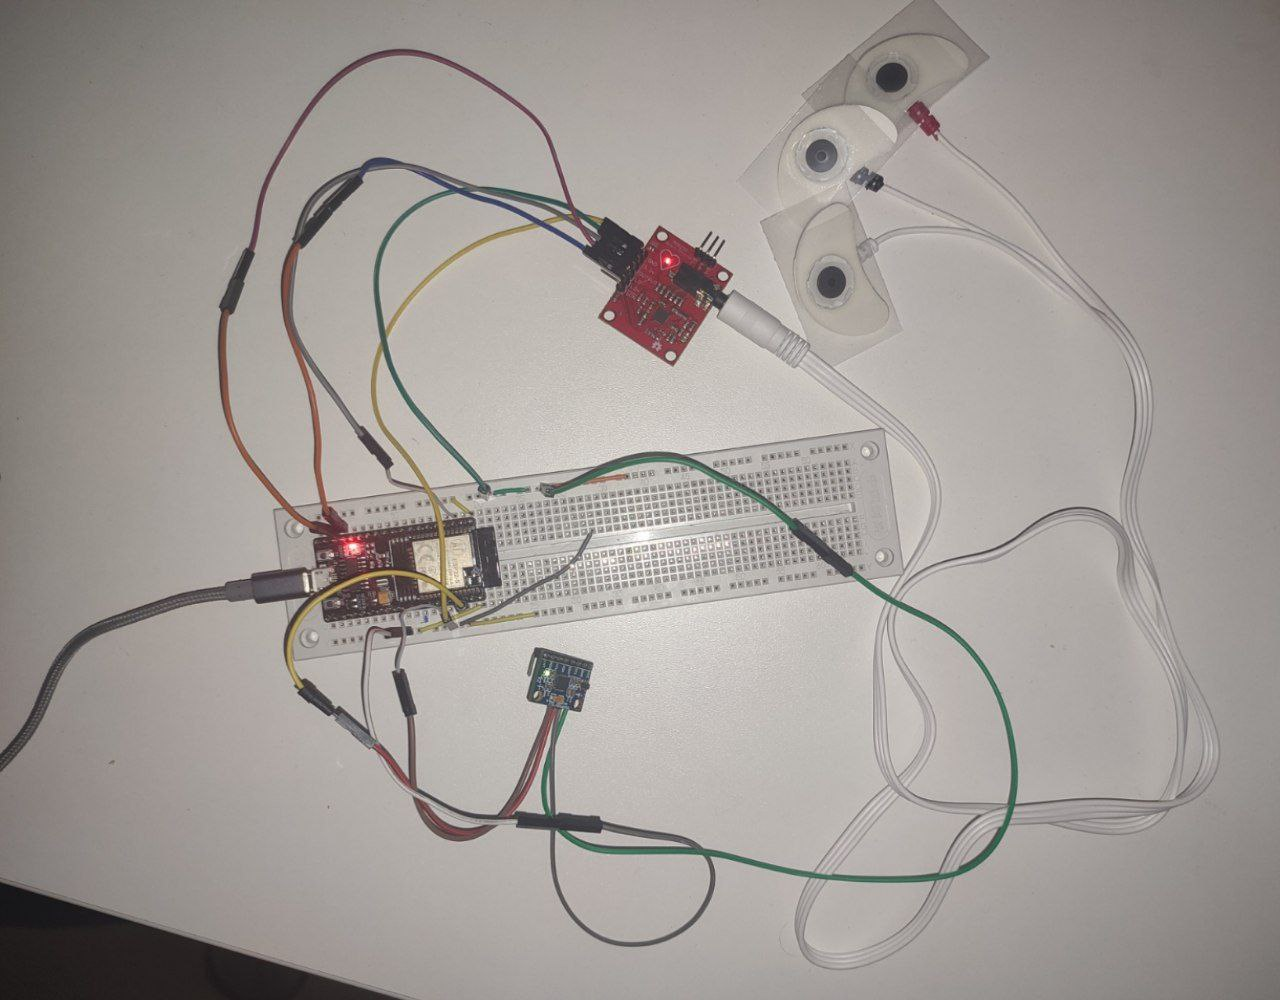
\includegraphics[width=1\linewidth]{Images/hardware.jpg}
    \caption{Wearable device hardware: an ESP32 microcontroller (left), an AD8232 ECG sensor (top), and an MPU6050 accelerometer (bottom)}
\end{figure}

I implemented the Wearable device firmware in the
Arduino~programming~language\footnote{\url{https://www.arduino.cc/reference/en/}} and
the Server software in the Python~programming~language\footnote{\url{https://python.org/}}
based on the
Flask~framework\footnote{\url{https://flask.palletsprojects.com/}}.
The software solution for the Intermediate device is based on the
\textit{ncat}\footnote{\url{https://nmap.org/ncat/}} and
\textit{curl}\footnote{\url{https://curl.se/}} open-source utilities.
\\

The source code for the~Wearable~device, the~Intermediate~device, and the~Server
is~available~at
\url{https://github.com/kolayne/dysphagia-project/tree/ERP}.
\\

The implemented system has a high level of reliability: because the Wearable device
communicates to the Intermediate device via the TCP protocol, it ensures that measurements
are delivered in order and without corruption; in case of connection failure the Wearable
device will retry sending data until the Intermediate device is up, so no data is lost.

\begin{figure}
    \centering
    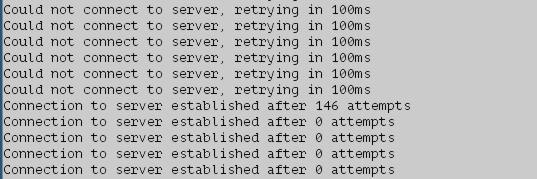
\includegraphics[width=1\linewidth]{Images/ESP: server down then up.jpg}
    \caption{Wearable device serial port log: the wearable device started before the Intermediate device was ready, so it keeps sending data until the endpoint is up, then continues normally}
\end{figure}

The Intermediate device, when sending data to the Server, can also detect successful
and failed submissions, as well as produce informative logs, which can be made visible
in the user interface to make the system more transparent for its users.

\begin{figure}
    \centering
    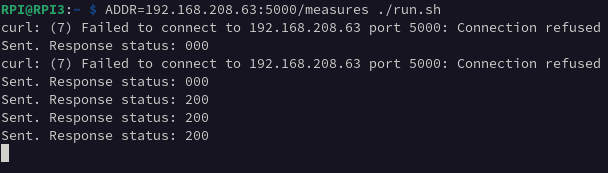
\includegraphics[width=1\linewidth]{Images/RPI: server down then up.png}
    \caption{Intermediate device command-line interface: the Intermediate device started before the Server was ready, so the first two requests failed with the error indicated; further requests succeeded}
\end{figure}

\section{Conclusion and future work}

In this project I implemented a prototype of the Wearable device based on the ESP32
controller and developed three software components that chain up devices of the system:
the Wearable device firmware that makes measurements and sends them via TCP,
the Intermediate device web server that accumulates data sent via TCP and forwards it via HTTP,
and the Server-side web server that accepts and decodes measurements sent via HTTP.
\\

Future work on the measurement collection system may continue in the following directions:
\begin{itemize}
    \item Adding more sensors to the Wearable device to collect more data relevant for analysis;
    \item Adding more data sources (e.g., connecting a video camera recording the patient);
    \item Improving security: adding authentication mechanisms to the Intermediate device and
          the Server, so that only data from the real device is collected and processed.
    \\
\end{itemize}

The results of this project can be used for collection of data from dysphagic patients in
further research of dysphagia in neurodegenerative diseases.



% \section*{References}
\FloatBarrier
\bibliographystyle{IEEEtran}
%\bibliography{./bibliography/IEEEabrv,./bibliography/IEEEexample}
\bibliography{./bibliography/IEEEabrv,contents/References/Bibliography}

\end{document}
